%%%%%%%%%%%%%%%%%%%%%%%%%%%%%%%%%%%%%%%%%
% University/School Laboratory Report
% LaTeX Template
% Version 4.0 (March 21, 2022)
%
% This template originates from:
% https://www.LaTeXTemplates.com
%
% Authors:
% Vel (vel@latextemplates.com)
% Linux and Unix Users Group at Virginia Tech Wiki
%
% License:
% CC BY-NC-SA 4.0 (https://creativecommons.org/licenses/by-nc-sa/4.0/)
%
%%%%%%%%%%%%%%%%%%%%%%%%%%%%%%%%%%%%%%%%%

%----------------------------------------------------------------------------------------
%	PACKAGES AND DOCUMENT CONFIGURATIONS
%----------------------------------------------------------------------------------------

\documentclass[
	a4paper, % Paper size, specify a4paper (A4) or letterpaper (US letter)
	10pt, % Default font size, specify 10pt, 11pt or 12pt
]{CSUniSchoolLabReport}


\addbibresource{sample.bib} % Bibliography file (located in the same folder as the template)

%----------------------------------------------------------------------------------------
%	REPORT INFORMATION
%----------------------------------------------------------------------------------------

\title{MA-CSEL \\ Conception systeme Embarqué Linux } % Report title

\author{Kirill \textsc{Goundiaev} \& Tanguy \textsc{Dietrich}} % Author name(s), add additional authors like: '\& James \textsc{Smith}'

\fancyhead[RE,LO]{Kirill Goundiaev \& Tanguy Dietrich}
\fancyhead[CE,CO]{\today}
\fancyhead[LE,RO]{MA-CSEL}

\fancyfoot[RE,LO]{MSE}
\fancyfoot[CE,CO]{\thepage} % this dicard page number dont touch
\fancyfoot[LE,RO]{HES-SO}
\date{\today} % Date of the report


% add image on the left top corner
% Definition of \maketitle
\makeatletter         
\def\@maketitle{
\raggedright
% 
\includegraphics[width = 60mm]{Figures/MSE.png}\\[8ex]

\includegraphics[width = 180mm]{Figures/ImageTitle.png}\\[8ex]
\begin{center}{}
{\Huge \@title }\\[4ex] 
{\Large  \@author}\\[4ex] 
\@date\\[8ex]
% 
\includegraphics[width = 40mm]{Figures/HESSO.png}
\end{center}}
\makeatother

%----------------------------------------------------------------------------------------

\begin{document}

\maketitle % Insert the title, author and date using the information specified above

% add an image
\begin{figure}[H] % Example image
\center{
\includegraphics[width=0.35\linewidth]{EMbeddedLinuxLogo}}
% \caption{Example image.}
\label{fig:speciation}
\end{figure}


%  to make a guard page
\newpage

% generate the summary table
\tableofcontents
\newpage


\section{Objectif}

This is my link: \footnote{\href{http://www.latex-tutorial.com}{http://www.latex-tutorial.com}}.

\section{Programmation Systeme}

\subsection{Systeme de fichier}\label{filesystem}

\subsection{Multiprocessing et Ordonnanceur}\label{multiprocess}
\subsubsection{Exercice 1 Processus et signaux}\label{MPEx1}
Le but de cet exercice etait de mettre en place une communication entre deux processus en utilisant un service linux tel que socketpair.
Le processus enfant devait envoyer des message au processus parent qui devait les afficher. Lorsque le process enfant envoie le message "exit" le programme doit se terminer.
Il etait aussi demander de fixer l'affinité des processus afin que le thread enfant effectue ces taches sur le CPU 1 et le thread parent sur le CPU 0.
Ainsi que d'ignorer les signaux SIGHUP, SIGINT, SIGQUIT, SIGABRT et SIGTERM.\\

Afin d'ignorer les signaux, nous avons utiliser la structure sigaction qui permet de modifier le comportement d'un signal.
Chaque handler de signal a été assigné a SIG\_IGN, ce qui permet d'ignorer le signal.
voici un extrait du code :

\begin{lstlisting}[style=CStyle, firstnumber=1]
	struct sigaction sa;
	sa.sa_handler = SIG_IGN;
	sigemptyset(&sa.sa_mask);
	sa.sa_flags = 0;
	sigaction(SIGHUP, &sa, NULL);
	sigaction(SIGINT, &sa, NULL);
	sigaction(SIGQUIT, &sa, NULL);
	sigaction(SIGABRT, &sa, NULL);
	sigaction(SIGTERM, &sa, NULL);
\end{lstlisting}
La création du socketpair se fait simplement avec ce bout de code :
\begin{lstlisting}[style=CStyle, firstnumber=1]
	int fd[2];
    if(socketpair(PF_LOCAL, SOCK_STREAM, 0, fd) < 0) {
        perror("socketpair");
        exit(1);
    }
\end{lstlisting}
Le paramentre PF\_LOCAL permet de créer un socket local, SOCK\_STREAM permet de créer un socket de type TCP. La valeur 0 permet de spécifier le protocole par défaut (ici TCP).

Afin de crée les deux process, nous avons utiliser la fonction fork() qui permet de crée un processus enfant identique au processus parent.
Voici un extrait du programme apres la fonction fork() :
\begin{lstlisting}[style=CStyle, firstnumber=1]
	pid = fork();
    if (pid == 0) { // child 
        close(fd[PARENTSOCKET]); 
        // set thread affinity
        if(setAffinity(1) == -1) { perror("sched_setaffinity");}
        child(fd[CHILDSOCKET]);
        close(fd[CHILDSOCKET]);
        exit(0);
    }
    else { // parent 
        close(fd[CHILDSOCKET]);
        // set thread affinity
        if(setAffinity(0) == -1) { perror("sched_setaffinity");}
        parent(fd[PARENTSOCKET]);
        close(fd[PARENTSOCKET]);
    }
    // must wait for child to exit
    // waitpid(pid, NULL, 0);
    wait(NULL);
\end{lstlisting}
La valeur de pid retourner par la fonction fork() permet de savoir si le processus est le parent ou l'enfant.
Ensuite il faut assigner l'affinité des processus, pour cela nous avons utiliser la fonction sched\_setaffinity() qui est appelé dans la fonction setAffinity() que nous avons créer.
Pour terminer il ne reste qu'as lancer la fonction correspondante au processus (enfant, ou parent).
Et ne pas oublier d'effectuer un wait pour attendre que le processus enfant se termine. Pour eviter les zombies.
La fonction setAffinity que nous avons créer utilise sched\_setaffinity, voici le code : \\
\begin{lstlisting}[style=CStyle, firstnumber=1]
	int setAffinity(int core) {
		// set thread affinity
		cpu_set_t cpuset;
		CPU_ZERO(&cpuset);
		// set this process to run on core 0
		CPU_SET(core, &cpuset);
		// here 0 mean use the calling process
		if(sched_setaffinity(0, sizeof(cpuset), &cpuset) == -1) {
	
			return -1;
		}
		return 0;
	}
\end{lstlisting}
La communication entre les deux process est assez simple etant donnée, que nous avons simplement 2 descripteur de fichier, du point de vue de notre programme, c'est comme si nous allions écrire/lire dans un fichier.
Il ne reste plus qu'as lire le descripteur de fichier dans le parent, et d'écrire avec l'enfant.\\
\noindent\begin{minipage}{.50\textwidth}
\begin{lstlisting}[style=CStyle, caption=Processus Enfant, firstnumber=1]{Name}
void child(int socket) {
	// get the child socket
	int cpt = 0;
	int messageLength;
	bool exitProcess = false;
	while (!exitProcess) {
		messageLength = strlen(messages[cpt])+1;
		write(socket,messages[cpt],messageLength);
		if (strcmp(messages[cpt], EXIT_MESSAGE) == 0) {
			exitProcess = true;
		}
		// juste to give the time to the parent to read the message
		// because the parent could read two message at once and not see the exit message
		usleep(1000000); 
		cpt = (cpt + 1) % NUM_MESSAGE;
	}
	printf("Child exit\r\n");
}
\end{lstlisting}
\end{minipage}\hfill
\begin{minipage}{.45\textwidth}
\begin{lstlisting}[style=CStyle, caption=Processus Parent, firstnumber=1]{Name}
void parent(int socket) {
	// get the parent socket
	char buffer[512];
	bool exitProcess = false;
	while (!exitProcess) {
		if(read(socket, buffer, sizeof(buffer)) <= 0) {
			perror("read");
			exit(1);
		}
		printf("Parent received: %s\r\n", buffer);
		if (strcmp(buffer, EXIT_MESSAGE) == 0) {
			exitProcess = true;
		}
	}
	printf("Parent exit\r\n");
}
\end{lstlisting}
\end{minipage}
Il faut tout de meme faire attention a plusieurs choses, premierement le parent peut recevoir deux message en meme temps avec la fonction read(), il faut donc faire attention a bien lire le message en entier.
Car on pourrait recevoir "message""exit", avec un zero terminal entre les deux. ce qui ferait que le programme ne s'arreterait pas.
Ensuite la taille du buffer pourrait ne pas etre suffisante pour lire le message en entier, ce qui pourrait crée un buffer overflow.\\

% Synthese de ce qui as été appris/exercé
Lors de ce TP, nous avons appris a utiliser les socketpair afin de communiquer entre deux processus.
Nous avons aussi appris a ignorer des signaux, mais il aurait aussi été possible de les rediriger vers une fonction. Dans le but d'effectuer une action.
Grace a ce TP, nous avons appris a gerer un processus (création, affinité, communication, etc...). En utilisant les fonction fork(), sched\_setaffinity(), socketpair(), etc...\\
% \linebreak

Ce labo a été plus compliquer que nous le pension, car nous avons eut de difficulté pour la reception du message "exit". La solution que nous avons choisit est simple mais pourrait poser des problemes.
Il serait mieux de regarder le nombre de bytes recu, et de parser le message recu dans different string, en utilisant les zero terminal.


\subsubsection{Exercice 2 CGroups Limitation memoire}\label{MPEx2}
% Exercice #2: Concevez une petite application permettant de valider la capacité des groupes de contrôle à limiter l’utilisation de la mémoire.
Dans cet exercice, l'objectif etait de montrer que les CGroups permettent de limiter l'utilisation de la memoire d'un processus.
Pour faire cela, nous avons créer un programme qui alloue de la memoire par block de 2MB, et qui rempli cette memoire avec des 0.
voici ce programme : \\
\begin{lstlisting}[style=CStyle, caption=Allocation de memoire, firstnumber=1]{Name}
	#define NUM_BLOCKS 50
	#define MEGABYTE 1024 * 1024
	#define BLOCK_SIZE (2 * MEGABYTE)
	
	int main(void)
	{
		int i;
		char *ptr[NUM_BLOCKS];
		printf("Allocating memory...\n");
		for (i = 0; i < NUM_BLOCKS; i++)
		{
			getchar();
			printf("Allocating block %d\n", i);
			ptr[i] = malloc(BLOCK_SIZE * sizeof(char));
			if (ptr[i] == NULL){exit(EXIT_FAILURE);}
			memset(ptr[i], 0, BLOCK_SIZE);
		}
		for (i = 0; i < NUM_BLOCKS; i++){free(ptr[i]);}
		return 0;
	}
\end{lstlisting}
Afin de voir ce qu'il ce passait, nous avons ajouter un print a chaque allocation pour voir a quel moment le programme serait stoppé.
Nous avons aussi ajouter un getchar() afin de pouvoir faire alloué un nouveau block de memoire.
\linebreak
avant de lancer ce code, il est necessaire de créer un groupe de controle, et de limiter la memoire de ce groupe. Afin de simplifier l'utilisation de ce programme, nous avons écrit un script qui permet de faire cela.

\begin{lstlisting}[language=bash, firstnumber=1]{Name}
#!/bin/sh
mount -t tmpfs none /sys/fs/cgroup
mkdir /sys/fs/cgroup/memory
mount -t cgroup -o memory memory /sys/fs/cgroup/memory
mkdir /sys/fs/cgroup/memory/mem
echo $$ > /sys/fs/cgroup/memory/mem/tasks
echo 20M > /sys/fs/cgroup/memory/mem/memory.limit_in_bytes
./ex2
\end{lstlisting}
Ce script monte un systeme de fichier tmpfs, puis monte un groupe de controle sur ce systeme de fichier.
Ensuite il cree un groupe de controle, et limite la memoire de ce groupe a 20MB a tout les processus qui y sont lié.
Enfin il lance le programme qui alloue de la memoire.

\begin{figure}[H]
	\centering
	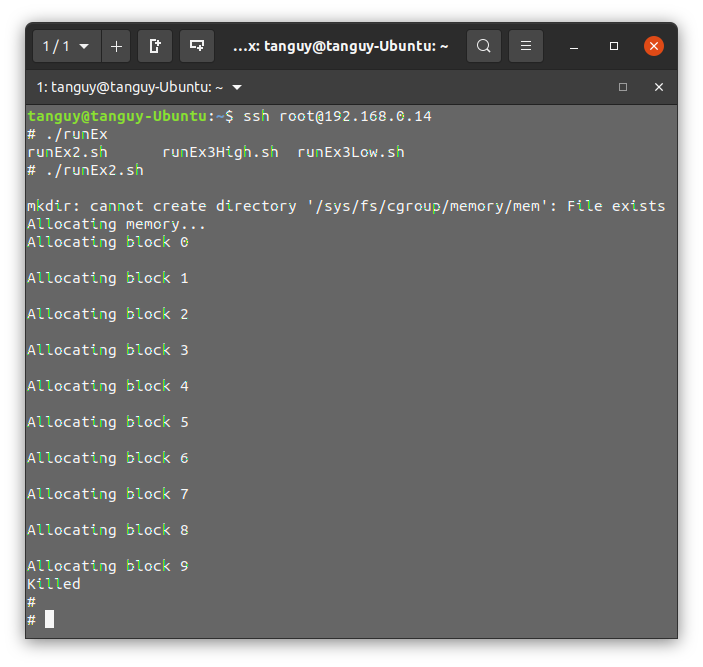
\includegraphics[width=0.4\linewidth]{runEx2}
	\caption{execution de l'exercice 2}
	\label{fig:ex2}
\end{figure}

Comme on peut le voir sur la figure \ref{fig:ex2}, le programme se fait tuer par le kernel lorsque l'on essaie d'allouer le 10eme block de memoire.
Ce qui correspond bien a la limite de 20MB que nous avons fixé.

\begin{enumerate}[label=\textbf{\arabic*}]
	\item \textbf{Quel effet a la commande echo \$\$ > ... sur les cgroups ?}\\
\$\$ en bash est le pid du processus courant. Donc cette commande permet d'écrire le pid du processus courant dans le fichier /sys/fs/cgroup/memory/mem/tasks. Ce qui permet de lier le processus courant au groupe de controle mem.
	
	\item \textbf{Quel est le comportement du sous-système memory lorsque le quota de mémoire est épuisé ? Pourrait-on le modifier ? Si oui, comment ?}\\
Lorsque le quota de memoire est epuisé, le kernel tue le processus qui a essayé d'allouer de la memoire.
Selon cette documentation \footnote{\href{https://access.redhat.com/documentation/en-us/red_hat_enterprise_linux/6/html/resource_management_guide/sec-memory}{https://access.redhat.com/documentation/en-us/red\_hat\_enterprise\_linux/6/html/resource\_management\_guide/sec-memory}}.
Il est possible de legerement modifier le comportement en utilisant le commande :
\begin{lstlisting}[language=bash, firstnumber=1]{Name}
	echo 1 > /sys/fs/cgroup/memory/mem/memory.oom_control
\end{lstlisting}
Cette commande desactive le "OOM Killer", si un programme atteint ça limite de memoire, il sera mis en pause j'usqu'a ce qu'il y ai de la memoire de disponible.

	\item \textbf{Est-il possible de surveiller/vérifier l’état actuel de la mémoire ? Si oui, comment ?}\\
Afin de surveiller la memoire, il y a plusieur options simple, comme la commande top, htop.
la fonction free permet aussi de voir l'etat de la memoire. Mais elle donne des informations sur la memoire globale, et non sur un processus en particulier.
Il est aussi possible de voir l'etat de la memoire d'un processus en utilisant la commande :
\begin{lstlisting}[language=bash, firstnumber=1]{Name}
	cat /proc/<PID>/stat | awk '{print $23}'
\end{lstlisting}
\end{enumerate}

% \linebreak

Nous ne conaission pas du tout les CGroups, ce qui a rendu cet exercice tres interessant.
Nous avons réussi a faire effectuer l'exercice, mais a un certain moment la limitation de memoire ne fonctionnait pas.
Il faudrai que l'on regarde plus en detail comment fonctionne les CGroups, et comment les utiliser, la structure et le nombre de fichier present dans le systeme de fichier /sys/fs/cgroup/memory/ est assez impressionant.
Toutefois, il est bon de savoir qu'il est possible de limiter la memoire d'un processus, et de voir comment cela fonctionne.

\subsubsection{Exercice 3 CGroups Controle du CPU}\label{MPEx3}
% Afin de valider la capacité des groupes de contrôle de limiter l’utilisation des CPU, 
% concevez une petite application composée au minimum de 2 processus utilisant le 100% des ressources du processeur.
Dans cet exercice, l'objectif est de limiter l'utilsation du CPU par un processus.
Pour cela, nous avons crée un programme qui lance 2 processus faisant des calcul afin de charger les CPU. 
Nous avons utiliser la fonction fork() vue dans l'exercice 1 (\ref{MPEx1}).

Ce programme nous permet de simplement lancer 2 processus qui vont charger les CPU.\\
\noindent\begin{minipage}{.50\textwidth}
	\begin{lstlisting}[style=CStyle, caption=Processus Enfant, firstnumber=1]{Name}
	int main(void)
	{
		pid_t pid;
		pid = fork();
		if (pid == 0) { // child
			compute();
			exit(0);
		}
		else { // parent
			compute();
		}
		// must wait for child to exit
		// waitpid(pid, NULL, 0);
		wait(NULL);
		return 0;
	}
	\end{lstlisting}
	\end{minipage}\hfill
	\begin{minipage}{.45\textwidth}
	\begin{lstlisting}[style=CStyle, caption=Processus Parent, firstnumber=1]{Name}
	void compute() {
		int a = 0;
		while (1) {
			// do some random computation
			a = (a + 1) % 1000000;
		}
	}
	\end{lstlisting}
\end{minipage}

Il reste a configurer les CGroups pour limiter l'utilisation du CPU par les processus. Pour faire cela, les ligne de commande nous ont été fourni.

\begin{lstlisting}[language=bash, firstnumber=1]{Name}
#!/bin/sh
mkdir /sys/fs/cgroup/cpuset
mount -t cgroup -o cpu,cpuset cpuset /sys/fs/cgroup/cpuset
mkdir /sys/fs/cgroup/cpuset/high
mkdir /sys/fs/cgroup/cpuset/low
echo 3 > /sys/fs/cgroup/cpuset/high/cpuset.cpus
echo 0 > /sys/fs/cgroup/cpuset/high/cpuset.mems
echo 2 > /sys/fs/cgroup/cpuset/low/cpuset.cpus
echo 0 > /sys/fs/cgroup/cpuset/low/cpuset.mems
echo $$ > /sys/fs/cgroup/cpuset/high/tasks
./ex3
\end{lstlisting}
Pour simplifier l'exercice, nous avons fait deux script bash, un qui lance le processus dans le groupe high, et un autre qui le lance dans le groupe low.
La seul difference se trouve a la ligne 10, ou nous changeons "high" en "low".


\begin{enumerate}[label=\textbf{\arabic*}]
	\item \textbf{Les 4 dernières lignes sont obligatoires pour que les prochaines commandes fonctionnent correctement. Pouvez-vous en donner la raison ?}\\
	La documentation trouvable ici : \footnote{\href{https://access.redhat.com/documentation/en-us/red_hat_enterprise_linux/6/html/resource_management_guide/sec-cpuset}{https://access.redhat.com/documentation/en-us/red\_hat\_enterprise\_linux/6/html/resource\_management\_guide/sec-cpuset}}
	nous indique que cpuset.cpus et cpuset.mems sont mandatoires pour chaque cgroup.
	le fichier cpuset.cpus permet de speficier sur quels CPU le processus peut s'executer, il est possible de specifier un intervalle de cpu, ou une liste.
	le fichier cpuset.mems permet de specifier quels noeud memoire le processus peut utiliser.
	
	
	Il est necessaire de specifier sur quelle CPU les processus vont s'executer
	\item \textbf{Ouvrez deux shells distincts et placez une dans le cgroup high et l’autre dans le cgroup low, par exemple :}\\
\begin{lstlisting}[language=bash, firstnumber=1]{Name}
$ ssh root@192.168.0.14
$ echo $$ > /sys/fs/cgroup/cpuset/low/tasks
\end{lstlisting}
\textbf{Lancez ensuite votre application dans chacun des shells. Quel devrait être le bon comportement ? Pouvez-vous le vérifier ?}\\
le programme appartenant au cgroupe high devrait tourner sur le CPU 3, alors que le programme appartenant au groupe low devrait tourner sur le CPU 2.
De plus comme un seul CPU est associé a 2 processus, le temps CPU devrait etre partagé entre les deux processus. la charge sera donc toujours de 100\% sur un CPU, mais partagé a 50\% entre les deux processus.
Afin de verifier cela, nous pouvons utiliser la commande htop, qui nous permet de voir l'utilisation des CPU.
Voici l'execution du script runEx3Low.sh :
\begin{figure}[H]
	\centering
	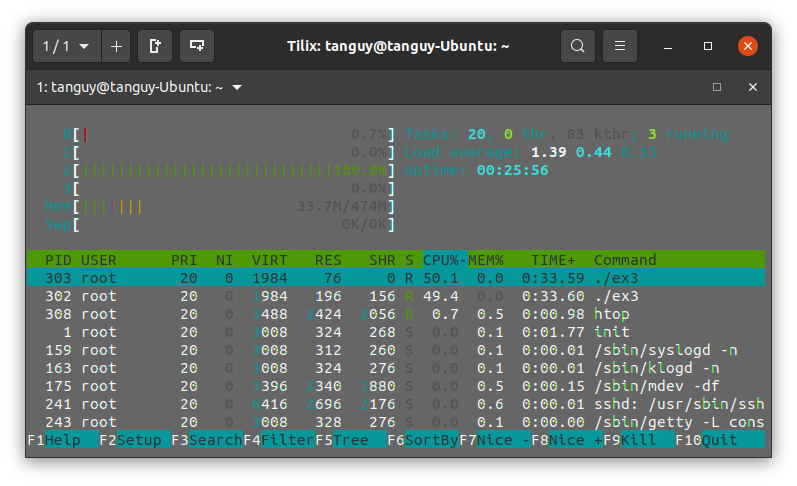
\includegraphics[width=0.7\linewidth]{MPEx3Low}
	\caption{Execution du script runEx3Low.sh}
	\label{fig:MPEx3Low}
\end{figure}
Sans arreter le script runEx3Low.sh, nous pouvons lancer le script runEx3High.sh :
\begin{figure}[H]
	\centering
	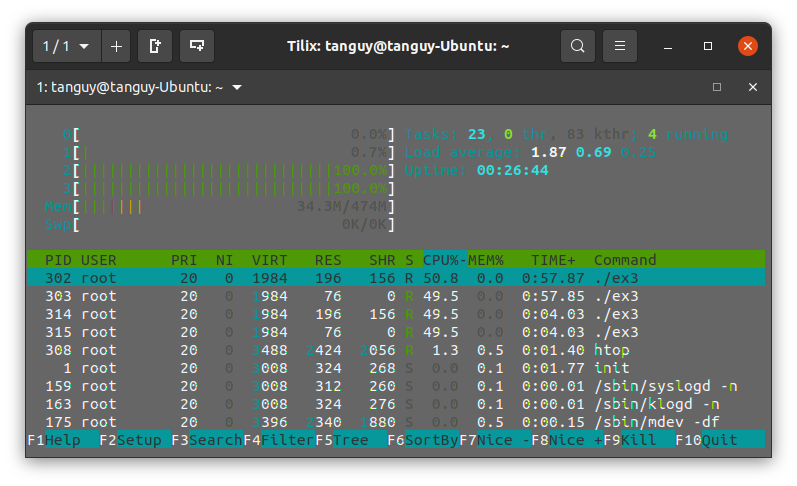
\includegraphics[width=0.7\linewidth]{MPEx3HighLow}
	\caption{Execution du script runEx3High.sh}
	\label{fig:MPEx3High}
\end{figure}

En modifiant la ligne 6 et 8, on peut faire en sorte que les processus se repartisse sur les 4 CPU, et non pas seulement 2.
\begin{lstlisting}[language=bash, firstnumber=1]{Name}
echo 2-3 > /sys/fs/cgroup/cpuset/high/cpuset.cpus
echo 0 > /sys/fs/cgroup/cpuset/high/cpuset.mems
echo 0-1 > /sys/fs/cgroup/cpuset/low/cpuset.cpus
echo 0 > /sys/fs/cgroup/cpuset/low/cpuset.mems
\end{lstlisting}

\begin{figure}[H]
	\centering
	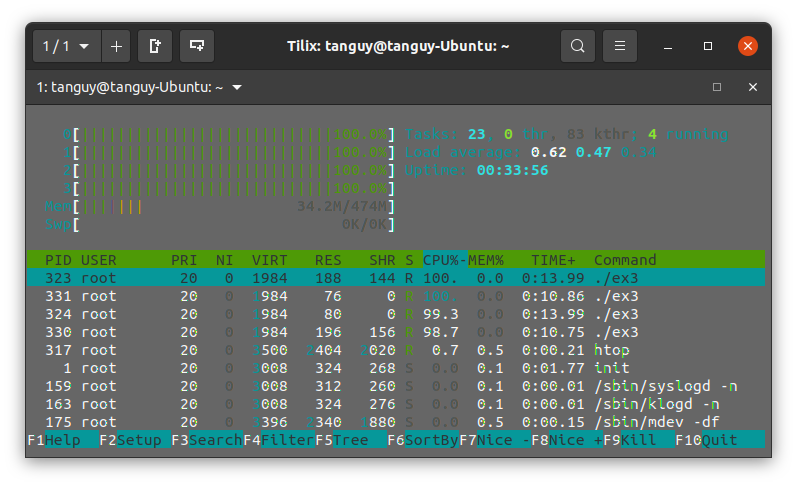
\includegraphics[width=0.7\linewidth]{MPEx3HighLow4CPU}
	\caption{Execution des deux scripts avec 4 CPU}
	\label{fig:MPEx3HighLow4CPU}
\end{figure}


	\item \textbf{Sachant que l’attribut cpu.shares permet de répartir le temps CPU entre différents cgroups, comment devrait-on procéder pour lancer deux tâches distinctes sur le cœur 4 de notre processeur et attribuer 75\% du temps CPU à la première tâche et 25\% à la deuxième ?}\\

Ici on veux faire tourner tous nos programme sur le CPU4, donc un peut ecrire.
\begin{lstlisting}[language=bash, firstnumber=1]{Name}
echo 3 > /sys/fs/cgroup/cpuset/high/cpuset.cpus
echo 0 > /sys/fs/cgroup/cpuset/high/cpuset.mems
echo 3 > /sys/fs/cgroup/cpuset/low/cpuset.cpus
echo 0 > /sys/fs/cgroup/cpuset/low/cpuset.mems
# set the cpu.shares
echo 768 > /sys/fs/cgroup/cpuset/high/cpu.shares
echo 256 > /sys/fs/cgroup/cpuset/low/cpu.shares
# change high to low for the other script
echo $$ > /sys/fs/cgroup/cpuset/high/tasks 
./ex3
\end{lstlisting}
Pour ce test, nous avons réutiliser le programme qui genere deux processus, nous aurons donc 2 processus qui se partageront 75\% du temps CPU, et deux autre pour les 25\% restant.
\begin{figure}[H]
	\centering
	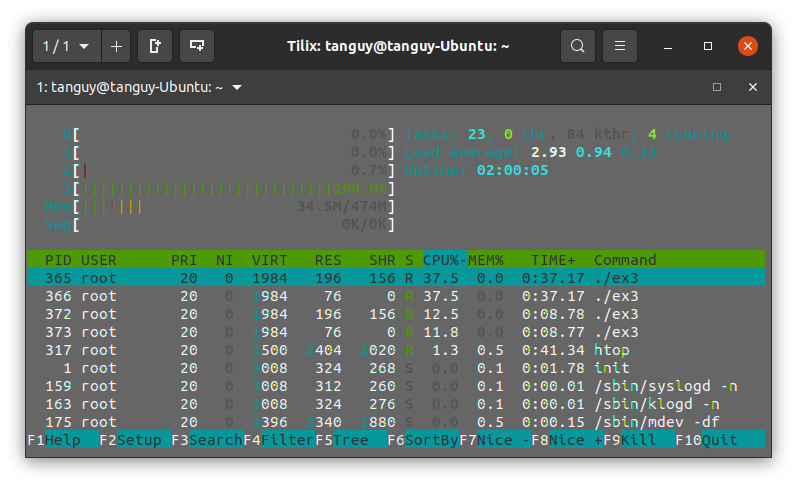
\includegraphics[width=0.7\linewidth]{runEx3Share}
	\caption{Execution des deux scripts avec 4 CPU}
	\label{fig:runEx3Share}
\end{figure}
On peut observer sur la figure \ref{fig:runEx3Share} que les deux processus on 37.5\% du temps CPU, et les deux autres 12.5\%.
ce qui fait bien 75\% et 25\%.

Ce TP etait tres proche du precedent, mais nous avons appris a gerer les ressource CPU alloué a un processus, et comment les partager entre plusieurs processus.
\end{enumerate}


\subsection{Outils d'analyse de performance pour Linux}
Dans cette partie, nous allons nous familiariser avec l'outil perf de Linux. Cet outil permet de mesurer les performances d'un programme. Il est possible de mesurer le temps d'execution d'un programme, le nombre de cycles d'horloge, le nombre d'instructions, le nombre de cache miss, etc.\\

tout d'abord, nous commencons par ajotuer binutils dans buildroot :
\begin{lstlisting}[language=bash, firstnumber=1]{Name}
$ cd /buildroot
$ make menuconfig
$ Target packages -> Development tools -> binutils
$ Target packages -> Development tools -> binutils binaries
$ make -j4
\end{lstlisting}

Puis nous installon le nouveau buildroot en prenant garde de ne pas effacer la configuration dans /etc/fstab, en utilisant les commande fournis dans le cours.
Apres avoir verifié que perfo soit bien installé, nous avons lancé la commande perf sur l'exercice 1 :
\begin{lstlisting}[language=bash, firstnumber=1]{Name}
$ perf stat ./ex1
\end{lstlisting}
Et nous avons obtenu le resultat suivant :
\begin{figure}[H]
	\centering
	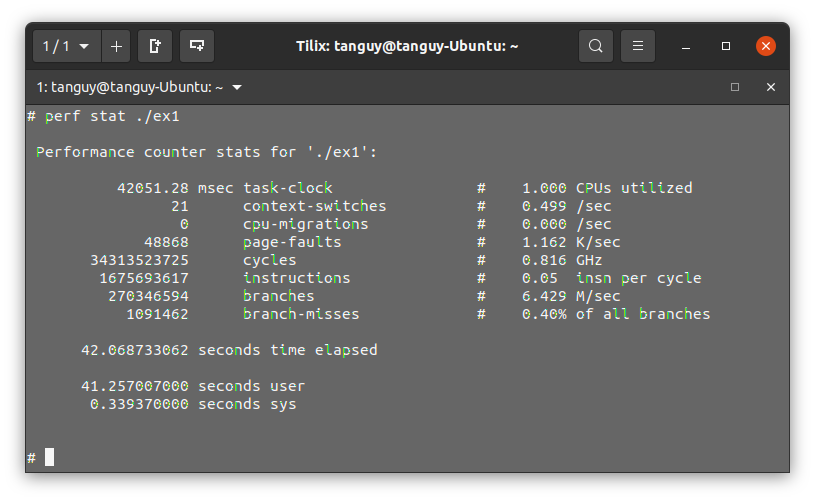
\includegraphics[width=0.7\linewidth]{perfEx1}
	\caption{Execution des deux scripts avec 4 CPU}
	\label{fig:runEx3Share}
\end{figure}

\begin{enumerate}[label=\textbf{\arabic*}]
	\item \textbf{Ce programme contient une erreur triviale qui empêche une utilisation optimale du cache. De quelle erreur s’agit-il ?}
L'erreur est que le tableau est parcuru en entier entre chaque increment, si tout le tableau rentrait dans la cache, cela pourrait ne pas poser de probleme.
Mais ici, le tableau est trop grand pour rentrer dans le cache, et donc a chaque increment, le cache est vidé, et le tableau est rechargé dans le cache, ce qui prend du temps.
Une modification simple pour rendre ce code plus efficace serait de deplacer la boucle d'increment a l'interieur des deux boucles.

\noindent\begin{minipage}{.45\textwidth}
	\begin{lstlisting}[style=CStyle, caption=Code fournis, firstnumber=1]{Name}
for (k = 0; k < 10; k++)
{
	for (i = 0; i < SIZE; i++)
	{
		for (j = 0; j < SIZE; j++)
		{
			array[j][i]++;
		}
	}
}
	\end{lstlisting}
	\end{minipage}\hfill
	\begin{minipage}{.45\textwidth}
	\begin{lstlisting}[style=CStyle, caption=Code modifié, firstnumber=1]{Name}
for (i = 0; i < SIZE; i++)
{
	for (j = 0; j < SIZE; j++)
	{
		for (k = 0; k < 10; k++)
		{
			// memory access already in cache
			array[j][i]++;
		}
	}
}
	\end{lstlisting}
\end{minipage}

Afin d'avoir un point de comparaison, nous avons lancé le programme de base avec la commande perf :
\begin{lstlisting}[language=bash, firstnumber=1]{Name}
$ perf stat -e cache-misses ./ex1
\end{lstlisting}
Et nous avons obtenu le resultat suivant :
\begin{figure}[H]
	\centering
	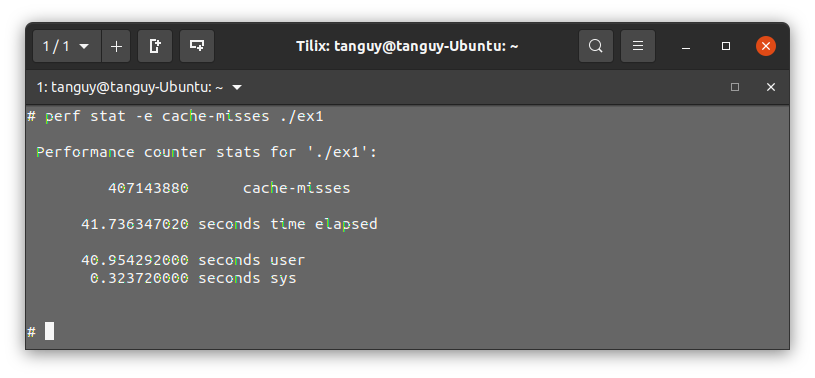
\includegraphics[width=0.7\linewidth]{perfEx1Cache}
	\caption{Execution des deux scripts avec 4 CPU}
	\label{fig:runEx3Share}
\end{figure}

	\item \textbf{Corrigez l’erreur, recompilez et mesurez à nouveau le temps d’exécution (soit avec perf stat, soit avec la commande time). Quelle amélioration constatez-vous ?}


Puis nous avons relancé le programme avec la correction :
\begin{figure}[H]
	\centering
	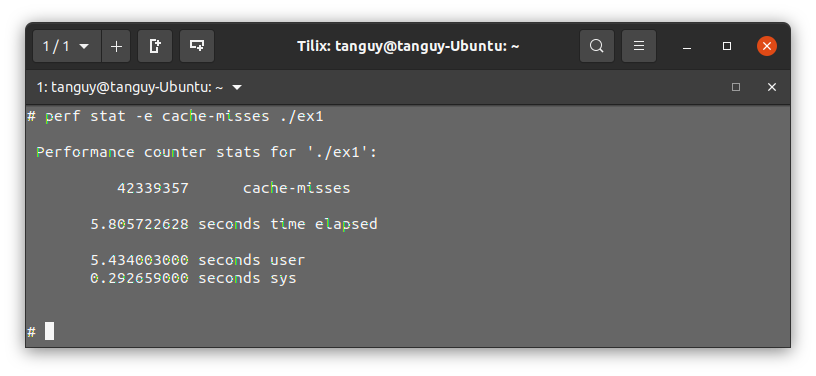
\includegraphics[width=0.7\linewidth]{perfEx1CacheOpti}
	\caption{Execution des deux scripts avec 4 CPU}
	\label{fig:runEx3Share}
\end{figure}
le temps est passé de 41.7s a 5.8s et le nombre de cache miss de 407143880 a 42339357. Il y a 9.6x moins de cache miss, et le temps d'execution est 7.2x plus rapide.\\
En modifiant une simple boucle

\item \textbf{Relevez les valeurs du compteur L1-dcache-load-misses pour les deux versions de l’application. Quel facteur constatez-vous entre les deux valeurs ?}

% array of two line and two column
\begin{center}
	\begin{tabular}{|c|c|c|}
		\hline
		& \textbf{Sans correction} & \textbf{Avec correction} \\
		\hline
		\textbf{L1-dcache-load-misses} & 406895610 & 42289308 \\
		\hline
		\textbf{cache-misses} & 407143880 & 42339357 \\
		\hline
	\end{tabular}
\end{center}
Les resultat sont similaire au deux resultat precedent, il y a 9.6x moins de cache miss, et le temps d'execution est 7.2x plus rapide.


\item \textbf{Décrivez brièvement ce que sont les évènements suivants :}
% add a sub-list to the question
\begin{enumerate}[label=\textbf{\alph*}]
	\item \textbf{instructions :} le nombre d'instruction executé
	\item \textbf{cache-misses :} le nombre de cache miss
	\item \textbf{branch-misses :} le nombre de branch miss
	\item \textbf{L1-dcache-load-misses :} le nombre de cache miss de niveau 1
	\item \textbf{cpu-migrations :} le nombre de migration de processus
	\item \textbf{context-switches :} le nombre de changement de contexte
\end{enumerate}

\item \textbf{Lors de la présentation de l’outil perf, on a vu que celui-ci permettait de profiler une application avec très peu d’impacts sur les performances. En utilisant la commande time, mesurez le temps d’exécution de notre application ex1 avec et sans la commande perf stat}\\
L'execution de la commande perf stat a pris 5.477 secondes, et l'execution de la commande time a pris 5.07 secondes. Mais il faudrait effectuer plusieur lancement pour avoir une moyenne plus precise.
On peut observer que le programme prend 0.4s de plus avec perf stat, ce qui est tres peu, et donc on peut dire que perf stat a tres peu d'impact sur les performances.

\end{enumerate}

% exercice 2
\textbf{Exercice 2 :}
\begin{enumerate}[label=\textbf{\arabic*}]

\item \textbf{Décrivez en quelques mots ce que fait ce programme.}\\
Le programme commence par remplir un tableau de 65536 entier avec des valeurs aléatoire entre 0 et 512 (en réalité les valeur ne sont pas aléatoire car la seed est toujorus la meme, la somme sera toujorus la meme).
Ensuite deux boucle for effectue 10000 fois la somme des valeur plus grande ou egale à 256.

\item \textbf{Mesurez le temps d’exécution}\\
Voici le resultat de l'execution du programme :


\begin{lstlisting}[language=bash, firstnumber=1]{Name}
# time ./ex2 
sum=125454290000
real	0m 26.19s
user	0m 26.11s
sys	0m 0.00s
\end{lstlisting}

Le programme prend 26,19 seconde pour s'executer.
dans le prochain test, nous allons essayer de trier le tableau en ajoutant ces ligne de code :
\begin{lstlisting}[style=CStyle, caption=Code modifié, firstnumber=1]{Name}
static int compare (const void* a, const void* b)
{
    return *(short*)a - *(short*)b;
}
qsort(array, SIZE, sizeof(short), compare);
\end{lstlisting}

Le temps est a present de 23.45 secondes, nous avons gagner 2.74 secondes.

\item \textbf{À l’aide de l’outil perf et de sa sous-commande stat, en utilisant différents compteurs déterminez pourquoi le programme modifié s’exécute plus rapidement.}\\

D'apres nos mesure, le gain de vitesse, viens des prediction de branchement.
Voici les resultat de perf stat : (les autre resultat sont assez similaire)\\
327884259      branch-misses             \#   33.17\% of all branches\\
842261         branch-misses             \#    0.08\% of all branches\\

Le fait que le tableau soit trié permet d'avoir de meilleur prediction de branchement, donc le pipeline est moins souvent cassé.
\end{enumerate}


% Exercice 3

\textbf{Exercice 3 :}
\begin{enumerate}[label=\textbf{\arabic*}]

\item \textbf{Compilez l’application et profilez l’application avec perf record :}\\
Nous executons la commande suivante :
\begin{lstlisting}[language=bash, firstnumber=1]{Name}
perf record --call-graph dwarf -e cpu-clock -F 75 \
./read-apache-logs access_log_NASA_Jul95_samples
\end{lstlisting}

un fichier report.data est généré, que nous analysons avec la commande suivante :
\begin{lstlisting}[language=bash, firstnumber=1]{Name}
perf report --no-children --demangle
\end{lstlisting}
\item \textbf{Avec les instructions précédentes, déterminez quelle fonction de notre application fait (indirectement) appel à std::operator==<char>.}\\

Le probleme viens de ce fonction :
\begin{lstlisting}[style=CStyle, caption=Extrait de hostcounter.cpp, firstnumber=1]{Name}
bool HostCounter::isNewHost(std::string hostname)
{
    return std::find(myHosts.begin(), myHosts.end(), hostname) == myHosts.end();
}
\end{lstlisting}

\item \textbf{Maintenant que vous savez quelle fonction utilise le plus de ressources CPU, trouvez une optimisation du code permettant de réduire drastiquement le temps d’exécution (vous devriez arriver à quelques dixièmes de secondes pour le fichier sample).}\\
Nous modifions le code afin d'utiliser la structure set, au lieu de vector et testons le temps d'exectution avec la commande time.
Le temps est a present de 1.49s, contre 2 minutes et 18 secondes avant la modification.
En executant a nouveau la commande perf record, nous pouvons voir que les fonction memcmp et cfree, sont les plus utilisé.

\item \textbf{Décrivez comment devrait-on procéder pour mesurer la latence et la gigue d’interruption, ceci aussi bien au niveau du noyau (kernel space) que de l’application (user space)}\\
Dans le cas d'un systeme embarqué avec une routine d'interuptions assigné a une pin, on pourrait envoyé un signal carré sur la pin d'interruption.
Puis inverser l'etat d'une pin de sortie, dans la routine d'interruption.
Ensuite a l'aide d'un oscilloscope, on pourrait mesurer la latence et la gigue d'interruption. en effectuant des moyenne, et en calculant l'ecart type.
\end{enumerate}


\section{Conclusion}

blabla

%----------------------------------------------------------------------------------------
%	BIBLIOGRAPHY
%----------------------------------------------------------------------------------------

\printbibliography % Output the bibliography

%----------------------------------------------------------------------------------------

\end{document}